\chapter{动物如何呼吸}\label{ch:g7:how-animals-breathe}

桥下的鳟鱼、草坪下的蚯蚓、
它上方的蜻蜓，以及站在草地上的你，
此刻都在做同一件事：从周围\omterm{def:g6:exploring-our-environment:components}{环境}中获取\omterm{def:g7:what-is-respiration:respiration}{氧气}
（\cref{def:g7:what-is-respiration:respiration}）。但你所处的\omterm{def:g6:exploring-our-environment:components}{环境}各不相同——
空气、\omterm{def:g6:decomposers-and-soil:soil}{土壤}、水——所用的\omterm{def:g7:what-is-respiration:respiration}{呼吸}装置也各不相同。
本章带你参观\omterm{def:g1:animals-around-us:animal}{动物}界的
各种\omterm{def:g7:what-is-respiration:respiration}{呼吸}装置。

\section{一个问题，四种装置}

\begin{proposition}[共同的设计规范]\label{prop:g7:how-animals-breathe:spec}
任何\omterm{def:g7:what-is-respiration:respiration}{呼吸}器官，无论属于哪种\omterm{def:g1:animals-around-us:animal}{动物}，都按同一规范构造，
这一规范此前已在
此前已在\cref{rem:g4:breathing:sponge}中见过：一个\emph{大}、\emph{薄}、
\emph{湿润}的表面，\omterm{def:g1:animals-around-us:animal}{动物}的\omterm{prop:g4:journey-of-food:absorb}{血液}（或体液）
足够接近周围\omterm{def:g6:exploring-our-environment:components}{环境}，使\omterm{def:g7:what-is-respiration:respiration}{氧气}得以
进入、\omterm{def:g7:what-is-respiration:respiration}{二氧化碳}排出。表面大，才有足够的交换量；
薄，便于气体通过；湿润，因为气体需要
溶解后才能通过。各类装置的差异在于其如何使该
表面与周围\omterm{def:g6:exploring-our-environment:components}{环境}相连接。
\end{proposition}
\admitted

\begin{definition}[四种呼吸装置]\label{def:g7:how-animals-breathe:four}
\omterm{def:g1:animals-around-us:animal}{动物}使其交换表面的方式主要有四种：
\begin{enumerate}
  \item \emph{肺}\index{肺}：充满空气的囊，折叠
        在\emph{体内}，由\omterm{def:g7:what-is-respiration:respiration}{呼吸}运动进行通气——
        \omterm{prop:g3:sorting-living-things:groups}{哺乳动物}、\omterm{prop:g3:sorting-living-things:groups}{鸟类}、\omterm{prop:g4:classifying-animals:classes}{爬行动物}、成体
        \omterm{prop:g3:sorting-living-things:groups}{两栖动物}；
  \item \emph{鳃}\index{鳃}：\omterm{def:g1:animals-around-us:covering}{羽毛}状的表面，
        位于\emph{体外或体缘}，
        由水流冲刷，见于\omterm{prop:g3:sorting-living-things:groups}{鱼类}
        （\cref{exo:g4:breathing:11}）、\omterm{ex:g2:animals-grow-up:frog}{蝌蚪}、许多水生
        幼虫、贻贝；
  \item \emph{气管}\index{气管（昆虫）}：一套细小的气管网络，
        由沿体侧分布的开口直接通往
        各器官——\omterm{prop:g3:sorting-living-things:groups}{昆虫}；空气被直接
        送到每个器官，很大程度上不依赖
        \omterm{prop:g4:journey-of-food:absorb}{血液}的帮助；
  \item \emph{皮肤呼吸}\index{皮肤呼吸}：整个湿润的
        \omterm{def:g1:the-five-senses:sense}{皮肤}作为交换表面——
        完全依靠\omterm{def:g1:the-five-senses:sense}{皮肤}的是蚯蚓；\omterm{prop:g3:sorting-living-things:groups}{两栖动物}则以\omterm{def:g1:the-five-senses:sense}{皮肤}作为
        简单肺的重要补充。
\end{enumerate}
\end{definition}

\begin{example}[观察装置运转]\label{ex:g7:how-animals-breathe:watch}
每种装置都有自己的节律。鳟鱼的口与鳃盖
交替有节奏地泵动：水从口进入，
流经鳃，再从鳃盖下排出。静止的蝗虫
腹部有节律地收缩——泵动其\omterm{def:g7:how-animals-breathe:four}{气管}。青蛙的
喉部颤动——把空气压入肺中，
（没有胸廓来完成这一过程）。只有蚯蚓看不出任何运动：
\omterm{def:g7:how-animals-breathe:four}{皮肤呼吸}完全没有运动，这正是
\cref{def:g7:what-is-respiration:respiration}区分气体交换与泵动
的原因。
\end{example}

\begin{omfigure}
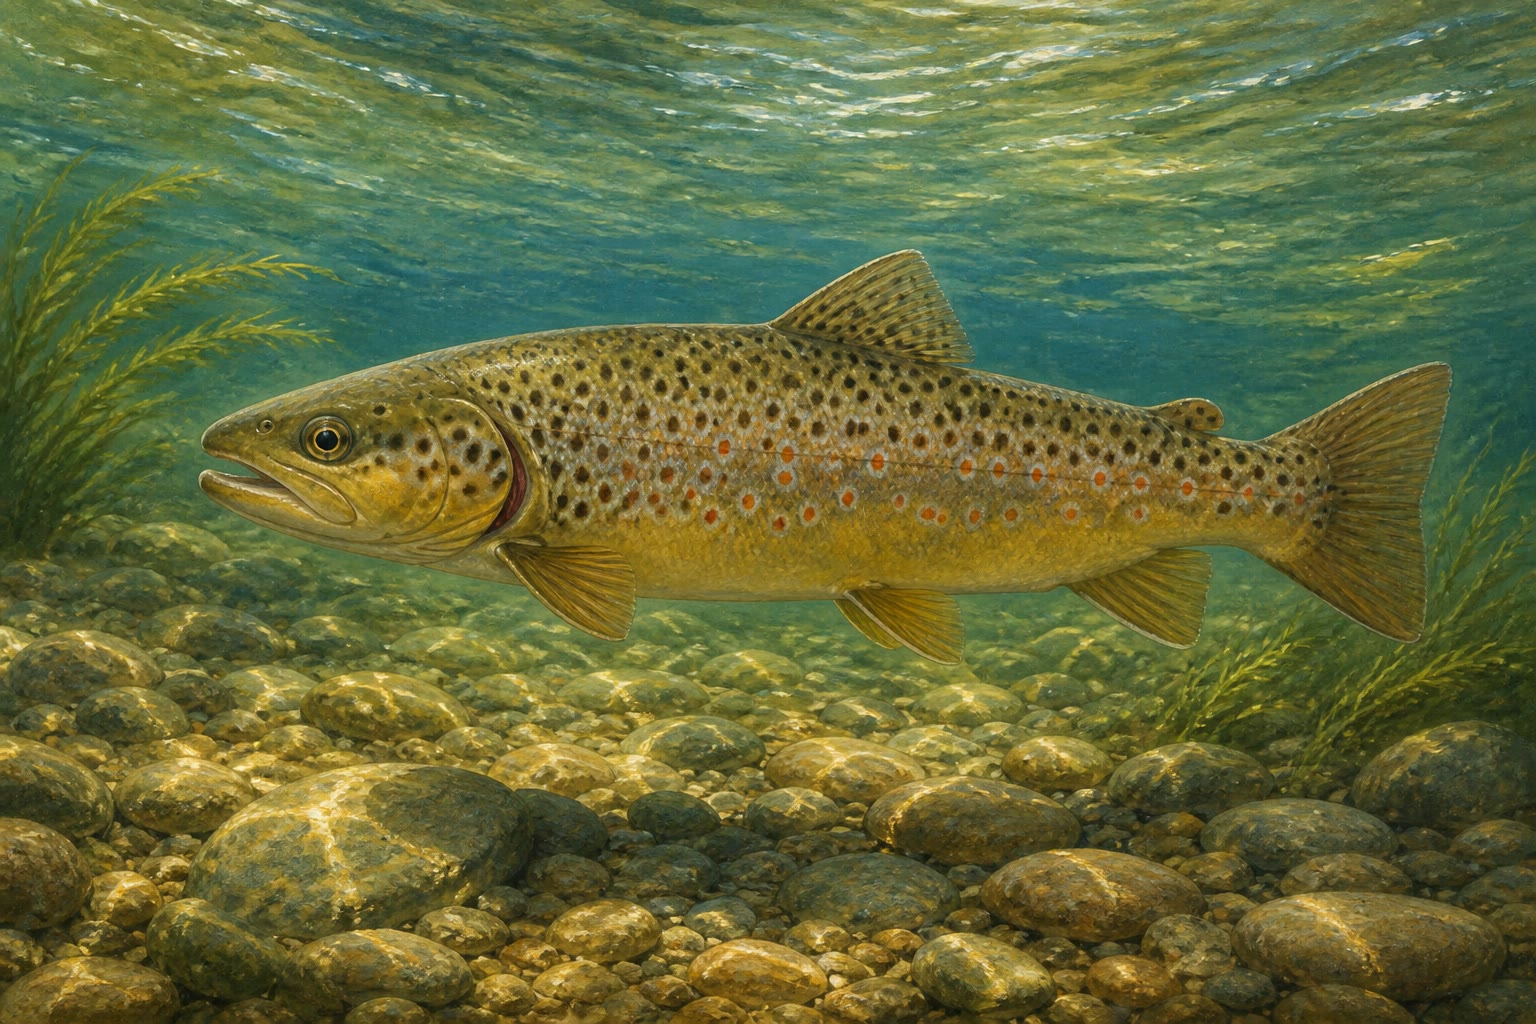
\includegraphics[width=0.6\linewidth]{images/book1/ai/g7-breathe-trout.jpg}

{\small 鳃式\omterm{def:g7:what-is-respiration:respiration}{呼吸}装置的主人：口与鳃盖
交替泵动单向水流，冲刷其\omterm{def:g1:animals-around-us:covering}{羽毛}状
交换表面。}
\end{omfigure}

\begin{omfigure}
\begin{tikzpicture}
  \node[anchor=south west, inner sep=0] (img) at (0,0)
    {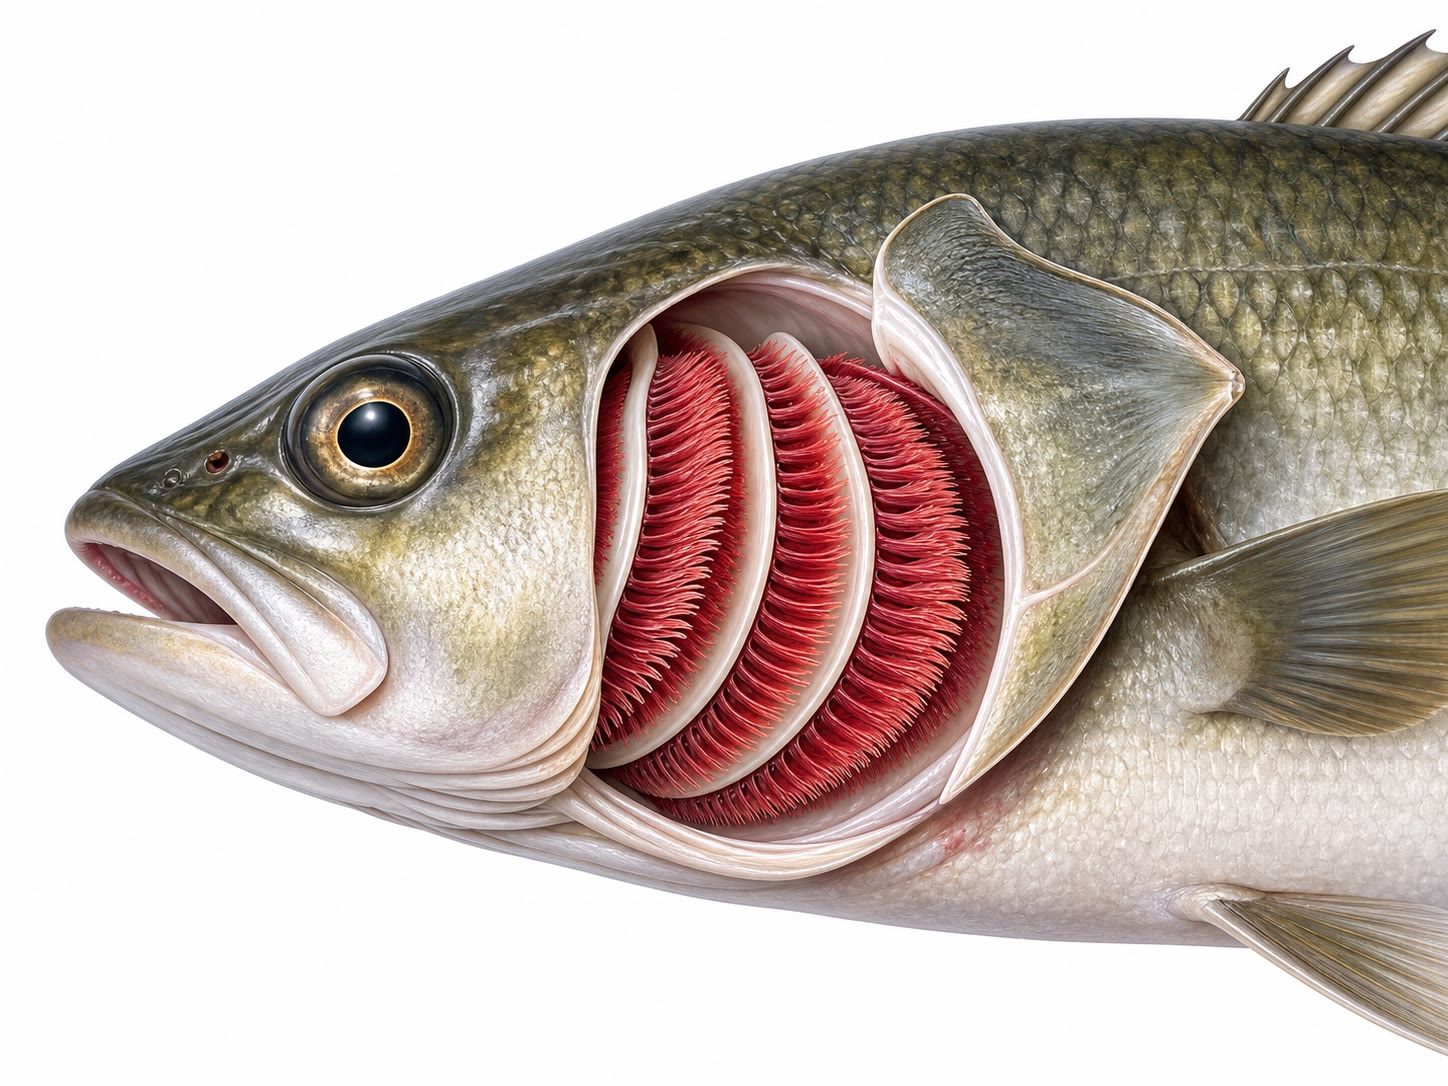
\includegraphics[width=0.56\linewidth]{images/book1/ai/fig-fish-gills.jpg}};
  \begin{scope}[x={(img.south east)}, y={(img.north west)},
      every node/.style={font=\small}]
    \draw[omDef, thick] (0.55,0.64) -- (0.32,0.92)
      node[above, align=center] {羽毛状的鳃，\\ 被水流冲刷};
    \draw[->, very thick, omDef] (-0.17,0.40) -- (0.02,0.40);
    \node[left, omDef] at (-0.18,0.40) {进水};
    \draw[->, very thick, omDef] (0.62,0.26) to[bend left=10] (0.70,-0.04);
    \node[below, omDef, align=center] at (0.70,-0.05)
      {出水，从 \\ 掀起的鳃盖下排出};
  \end{scope}
\end{tikzpicture}

{\small 鳃式\omterm{def:g7:what-is-respiration:respiration}{呼吸}装置（去除鳃盖）：单向水流从
口进入，冲刷\omterm{def:g1:animals-around-us:covering}{羽毛}状的红色鳃弓，然后
从鳃盖下离开。}
\end{omfigure}

\section{装置适应介质与生活方式}

\begin{proposition}[各装置各适其所]\label{prop:g7:how-animals-breathe:fits}
各类装置与介质和生活方式
（\cref{def:g4:adapted-to-their-world:adaptation}在\omterm{def:g7:what-is-respiration:respiration}{呼吸}方面的体现）：
在\omterm{def:g7:what-is-respiration:respiration}{呼吸}方面的体现）：
\begin{itemize}
  \item 鳃适于水中：其\omterm{def:g1:animals-around-us:covering}{羽毛}状表面在水中
        彼此分开，持续受水流冲刷——而在空气中
        会无效地塌陷（\cref{exo:g4:breathing:11}中
        窒息的鳟鱼）；
  \item 肺适于空气：折叠于体内，保持湿润
        使水分不致像在开放水体中那样流失——但它们无法
        获取水中稀少的溶解氧；
  \item \omterm{def:g7:how-animals-breathe:four}{气管}适于小型身体：在毫米级距离上效果极佳，
        但在长距离上输送过慢，
        这也是\omterm{prop:g3:sorting-living-things:groups}{昆虫}体型较小的原因之一；
  \item \omterm{def:g7:how-animals-breathe:four}{皮肤呼吸}适于体型小、\omterm{def:g1:the-five-senses:sense}{皮肤}湿润的\omterm{def:g6:exploring-our-environment:components}{生物}，生活在
        潮湿\omterm{def:g6:exploring-our-environment:components}{环境}中：蚯蚓的整个体表几乎
        仅够其纤薄的身体所用，干燥空气会使其死亡——
        想想雨后搁浅的蚯蚓吧。
\end{itemize}
\end{proposition}
\admitted

\begin{example}[一种动物的两段生活，两套呼吸机制]\label{ex:g7:how-animals-breathe:frog}
青蛙一生中贯穿了本章的全部内容：\omterm{ex:g2:animals-grow-up:frog}{蝌蚪}时期以鳃\omterm{def:g7:what-is-respiration:respiration}{呼吸}
（水中生活的机制，
\cref{ex:g2:animals-grow-up:frog}），兼用肺与湿润\omterm{def:g1:the-five-senses:sense}{皮肤}，
成体——肺结构简单，\omterm{def:g1:the-five-senses:sense}{皮肤}承担了大部分
工作，尤其是在寒冷的池底越冬期间
（\cref{exo:g6:life-through-seasons:11}：那只\omterm{def:g3:animals-through-seasons:hibernation}{冬眠}的青蛙
仅靠\omterm{def:g7:how-animals-breathe:four}{皮肤呼吸}）。\omterm{def:g2:animals-grow-up:metamorphosis}{变态}发育重新塑造了
甚至包括\omterm{def:g7:what-is-respiration:respiration}{呼吸}机制。
\end{example}

\begin{example}[在水中生活却要呼吸空气]\label{ex:g7:how-animals-breathe:airinwater}
用肺\omterm{def:g7:what-is-respiration:respiration}{呼吸}的水生\omterm{def:g1:animals-around-us:animal}{动物}必须往返于水面与水下。海豚和
鲸要浮出水面喷气、\omterm{def:g4:breathing:movements}{吸气}
（\cref{ex:g6:classification-kinship:whale}：\omterm{prop:g3:sorting-living-things:groups}{哺乳动物}的肺，
由陆生祖先遗传而来）；池塘螺则爬到
水面补充空气；龙虱则在翅鞘下携带一个银色
气泡——好比潜水员的气瓶，
在水面处补充更新。\omterm{def:g2:where-animals-live:habitat}{栖息地}可以改变，
但机制所依赖的介质不能改变。
\end{example}

\begin{method}[读懂动物的呼吸方式]\label{met:g7:how-animals-breathe:read}
对于一种不熟悉的\omterm{def:g1:animals-around-us:animal}{动物}，可按以下步骤进行：
\begin{enumerate}
  \item 它生活在哪里——能否离开？（水中、
        空气中、\omterm{def:g6:decomposers-and-soil:soil}{土壤}中；往返型或定居型）；
  \item 寻找\omterm{def:g7:what-is-respiration:respiration}{呼吸}机制的特征：鳃盖，或
        羽状鳃丝；鼻孔与可起伏的胸部；
        沿\omterm{prop:g3:sorting-living-things:groups}{昆虫}身体排列的一列列微小开口；或
        除湿润的\omterm{def:g1:the-five-senses:sense}{皮肤}外别无可见结构；
  \item 观察节律：鳃盖的开合、腹部的搏动、
        胸部的起伏、浮出水面的次数；
  \item 确定\omterm{def:g7:what-is-respiration:respiration}{呼吸}机制的类型——并与
        介质是否相符，依据
        \cref{prop:g7:how-animals-breathe:fits}检验。
\end{enumerate}
\end{method}

\begin{remark}[共同要求从不改变]\label{rem:g7:how-animals-breathe:same}
无论形式多么多样，仔细观察四种机制中的任何一种，
都会看到\cref{prop:g7:how-animals-breathe:spec}再次出现：
鳃丝、肺泡与\omterm{def:g7:how-animals-breathe:four}{气管}的末梢，
以及蚯蚓的\omterm{def:g1:the-five-senses:sense}{皮肤}，它们都是大面积、薄而湿的
外界与身体的接触面。四种机制，
同一套要求——\omterm{prop:g5:first-look-at-cells:principle}{生命的统一性}
（\cref{prop:g5:first-look-at-cells:principle}），
体现在\omterm{def:g7:what-is-respiration:respiration}{呼吸}器官上。
\end{remark}

\section{练习}

\begin{exercise}[$\star$]\label{exo:g7:how-animals-breathe:1}
说明每种\omterm{def:g7:what-is-respiration:respiration}{呼吸}器官都需满足的共同要求，
以及这三个特性各自为何重要。
\end{exercise}

\begin{exercise}[$\star$]\label{exo:g7:how-animals-breathe:2}
说出四种\omterm{def:g7:what-is-respiration:respiration}{呼吸}机制，并各举出两种使用该机制的\omterm{def:g1:animals-around-us:animal}{动物}。
\end{exercise}

\begin{exercise}[$\star$]\label{exo:g7:how-animals-breathe:3}
描述虹鳟的泵水过程：水流入、流经
与流出的路径。
\end{exercise}

\begin{exercise}[$\star$]\label{exo:g7:how-animals-breathe:4}
\omterm{prop:g3:sorting-living-things:groups}{昆虫}没有肺，它们如何输送\omterm{def:g7:what-is-respiration:respiration}{氧气}——
在很大程度上不借助\omterm{prop:g4:journey-of-food:absorb}{血液}的帮助？
\end{exercise}

\begin{exercise}[$\star$]\label{exo:g7:how-animals-breathe:5}
为什么搁浅的虹鳟在富含\omterm{def:g7:what-is-respiration:respiration}{氧气}的空气中会窒息？
\end{exercise}

\begin{exercise}[$\star$]\label{exo:g7:how-animals-breathe:6}
为什么干燥的阳光会使人行道上的蚯蚓死亡？
哪种\omterm{def:g7:what-is-respiration:respiration}{呼吸}机制失效了？如何失效？
\end{exercise}

\begin{exercise}[$\star\star$]\label{exo:g7:how-animals-breathe:7}
列出青蛙一生中所用的\omterm{def:g7:what-is-respiration:respiration}{呼吸}机制，
并注明每种机制对应的季节或发育阶段。
\end{exercise}

\begin{exercise}[$\star\star$]\label{exo:g7:how-animals-breathe:8}
海豚的生活方式像鱼，却会像人一样溺水。
请结合\omterm{def:g7:what-is-respiration:respiration}{呼吸}机制与祖先关系加以解释
（见\cref{ex:g6:classification-kinship:whale}）。
\end{exercise}

\begin{exercise}[$\star\star$]\label{exo:g7:how-animals-breathe:9}
龙虱身上银色的气泡是什么？它必须
定期对它做什么？
\end{exercise}

\begin{exercise}[$\star\star$]\label{exo:g7:how-animals-breathe:10}
用\cref{met:g7:how-animals-breathe:read}分析：(a) 一只
贻贝；(b) 蝗虫；(c) 一条草蛇，
正游过池塘。
\end{exercise}

\begin{exercise}[$\star\star$]\label{exo:g7:how-animals-breathe:11}
为什么不存在鲸那么大的\omterm{prop:g3:sorting-living-things:groups}{昆虫}？请结合
\omterm{def:g7:how-animals-breathe:four}{气管}的极限作答。
\end{exercise}

\begin{exercise}[$\star\star\star$]\label{exo:g7:how-animals-breathe:12}
“四种机制，同一套要求。”请为这句话辩护：
说明共同的要求，并说明鳃、肺、
\omterm{def:g7:how-animals-breathe:four}{气管}和\omterm{def:g1:the-five-senses:sense}{皮肤}各自如何满足其三项要求。
\end{exercise}

\section{问题：池塘里的呼吸者普查}

\begin{problem}[{周末问题——一个池塘，
每台机器都在工作}]\label{pb:g7:how-animals-breathe:1}
一个下午，带着网、观察箱和
笔记本。普查对象有：鳟鱼苗和刺鱼；\omterm{ex:g2:animals-grow-up:frog}{蝌蚪}
（有些长出了后腿）；成年青蛙；在水面膜上爬行的池塘田螺；
一只闪着银光的龙虱；
石块下带羽状丛毛的蜉蝣幼虫；以及
河岸潮湿草坪上的蚯蚓。

\medskip\noindent\textbf{第一部分——给各种\omterm{def:g7:what-is-respiration:respiration}{呼吸}机制命名。}
\begin{enumerate}
  \item 为普查中的每种\omterm{def:g6:exploring-our-environment:components}{生物}指定其\omterm{def:g7:what-is-respiration:respiration}{呼吸}机制。
  \item 蜉蝣幼虫的羽状丛毛即使在静水中也不停地摆动。
        这些丛毛是什么结构？摆动的作用是
        什么？
  \item 哪些普查对象必须到水面去，
        以及为什么恰好是它们？
  \item 无后腿的\omterm{ex:g2:animals-grow-up:frog}{蝌蚪}与有后腿的\omterm{ex:g2:animals-grow-up:frog}{蝌蚪}，
        内部结构的差异可能与外部一样大。
        正在进行的是哪种改建，
        根据\cref{ex:g7:how-animals-breathe:frog}？
\end{enumerate}

\medskip\noindent\textbf{第二部分——承压下的
\omterm{def:g7:what-is-respiration:respiration}{呼吸}机制。}
\begin{enumerate}[resume]
  \item 闷热无风的一周使池塘中的溶解氧
        含量降低（\cref{ch:g7:oxygen-in-the-water}将
        解释其原因）。请为普查对象排序：谁最先受害——
        用鳃\omterm{def:g7:what-is-respiration:respiration}{呼吸}的\omterm{def:g1:animals-around-us:animal}{动物}，还是往返水面的\omterm{def:g1:animals-around-us:animal}{动物}？
        为什么？
  \item 那一周，刺鱼悬停在水面之下，
        嘴巴贴着水膜一张一合。
        请用规范解释这一行为：
        水面最上层一毫米有何特别之处？
  \item 一位粗心的涉水者搅起大片细泥。哪一种
        \omterm{def:g7:what-is-respiration:respiration}{呼吸}机制会被堵塞？你预计受影响的\omterm{def:g1:animals-around-us:animal}{动物}
        会有什么表现？
  \item 夜间下过雨后，草坪上的蚯蚓
        纷纷爬到小路上。请解释这一经典景象：
        哪种机制、哪种\omterm{def:g6:exploring-our-environment:conditions}{条件}驱使它们
        爬出地面？
\end{enumerate}

\medskip\noindent\textbf{第三部分——更大的图景。}
\begin{enumerate}[resume]
  \item 将普查结果列成表格：\omterm{def:g1:animals-around-us:animal}{动物}、机制、介质、
        往返或常驻。哪一条单一规范
        位于每一机制栏之首，
        据\cref{rem:g7:how-animals-breathe:same}？
  \item 池塘在一月结冰，封住了
        水面。预测冬季的命运：青蛙
        （\cref{exo:g6:life-through-seasons:11}）、
        田螺、龙虱、\omterm{prop:g3:sorting-living-things:groups}{鱼类}——谁陷入困境，
        谁早已有所准备？
  \item 一位新来者登场：一只水蜘蛛，
        它编织丝质的“钟罩”，并在其中储存水面空气。请把
        它的本领与龙虱的并列比较，
        并指出它持续服务的是哪种机制。
  \item 作总结：为什么一个小小的池塘需要
        四种不同的\omterm{def:g7:what-is-respiration:respiration}{呼吸}机制，才能被完整地栖居？
        用一句话作答，须用到\emph{介质}和
        \emph{\omterm{def:g7:what-is-respiration:respiration}{氧气}}。
\end{enumerate}
\end{problem}
